%
% File emnlp2019.tex
%
%% Based on the style files for ACL 2019, which were
%% Based on the style files for EMNLP 2018, which were
%% Based on the style files for ACL 2018, which were
%% Based on the style files for ACL-2015, with some improvements
%%  taken from the NAACL-2016 style
%% Based on the style files for ACL-2014, which were, in turn,
%% based on ACL-2013, ACL-2012, ACL-2011, ACL-2010, ACL-IJCNLP-2009,
%% EACL-2009, IJCNLP-2008...
%% Based on the style files for EACL 2006 by 
%%e.agirre@ehu.es or Sergi.Balari@uab.es
%% and that of ACL 08 by Joakim Nivre and Noah Smith

\documentclass[11pt,a4paper]{article}
\usepackage[hyperref]{emnlp-ijcnlp-2019}
\usepackage{times}
\usepackage{latexsym}
\usepackage{amsmath,epsfig,amsfonts,dsfont}
\usepackage{booktabs, multirow}
\usepackage{url}
\usepackage{soul}
\DeclareMathOperator{\avg}{avg}
\DeclareMathOperator{\mean}{mean}
\DeclareMathOperator{\ReLU}{ReLU}
\DeclareMathOperator{\merge}{Agg}





%\aclfinalcopy % Uncomment this line for the final submission

%\setlength\titlebox{5cm}
% You can expand the titlebox if you need extra space
% to show all the authors. Please do not make the titlebox
% smaller than 5cm (the original size); we will check this
% in the camera-ready version and ask you to change it back.

\newcommand\BibTeX{B{\sc ib}\TeX}
\newcommand\confname{EMNLP-IJCNLP 2019}
\newcommand\conforg{SIGDAT}
\newcommand{\KZ}[1]{\textcolor{blue}{Kenny: #1}}
\newcommand{\KH}[1]{\textcolor{purple}{Kelsey: #1}}
\newcommand{\secref}[1]{Section \ref{#1}}
\newcommand{\figref}[1]{Figure \ref{#1}}
\newcommand{\eqnref}[1]{Eq. (\ref{#1})}
\newcommand{\tabref}[1]{Table \ref{#1}}
\newcommand{\exref}[1]{Example \ref{#1}}
\newcommand{\cut}[1]{}
\newcommand{\tabincell}[2]{\begin{tabular}{@{}#1@{}}#2\end{tabular}}

\title{Question Generation from Text using Syntactic Structure Information}

\author{First Author \\
  Affiliation / Address line 1 \\
  Affiliation / Address line 2 \\
  Affiliation / Address line 3 \\
  {\tt email@domain} \\\And
  Second Author \\
  Affiliation / Address line 1 \\
  Affiliation / Address line 2 \\
  Affiliation / Address line 3 \\
  {\tt email@domain} \\}

\date{}

\begin{document}
\maketitle
\begin{abstract}
Textual question generation is a task 
of generating meaningful questions about an input text with a key phrase. 
Much previous work focuses on neural models that treat the input text 
as a sequence of words. In this paper, we propose to view the text as 
both a sequence of words and a structure of syntactic components.
We develop a model that takes advantage of the parse tree of the text, 
and results show that this model outperforms the seq-to-seq model and basic tree-to-seq model
substantially. 
\end{abstract}

%\IEEEraisesectionheading{
% %\IEEEraisesectionheading{
% %\IEEEraisesectionheading{
% \input{intro}
\section{Introduction}\label{sec:intro}
 %}
% \section{Introduction}\label{sec:intro}

% \begin{enumerate}
% \item Motivation: application scenarios (with 1-2 running examples);
% \item Characteristics of the data sources and their challenges;
% \item Briefly introduce previous approaches to extract information 
% from images including setting the document zone, and their limitations.
% \item General flow of our approach (may give a diagram here)
% \end{enumerate}
% scenary

Due to ever evolving hardware and software, many medical images
such as electro-cardio graphs (ECGs), X-ray or ultrasound images  
are directly printed and stored in hard copy formats. 
% \KZ{Insert 4 example images here.}
%Examples are shown in \figref{fig:medicalImages}. 
% These images often contain a mix of graphics and text, which
% include parameter settings of the hardware, test measurements or simple
% diagnosis. 
These images often contain a mix of graphics and text, which 
include technical settings of the hardware used, test measurements or simple diagnoses.
Recently, there has been a growing demand for digitizing such 
medical information from paper media sources, especially legacy ones, or patients who want to keep track of these documents by themselves digitally. 
Apart from scanning the graphics into a digital format, extracting 
the semi-structured textual information is also an important part of
building electronic medical records for patients. 

%\begin{figure}[!htb]
%\centering
%\subfloat[ECG]{
%\label{fig:medicalimage:ecg}
%\epsfig{file=figure/17_ori.eps, width=0.4\columnwidth}
%}
%% \hfill
%\subfloat[MRI]{
%	\label{fig:medicalimage:mrt}
%	\epsfig{file=figure/MRI.eps, width=0.4\columnwidth}
%}
%\\
%\subfloat[X-RAY]{
%\label{fig:medicalimage:xray}
%\epsfig{file=figure/X-RAY.eps, width=0.4\columnwidth}
%}
%%\hfill
%\subfloat[EEG]{
%\label{fig:medicalimage:eeg}
%\epsfig{file=figure/EEG.eps, width=0.4\columnwidth}
%}
%\caption{Examples of Medical Images}
%\label{fig:medicalImages}
%\end{figure}

Optical character recognition (OCR)  \cite{mori1992historical,smith2007overview} is 
a traditional technique used to turn images of printed text into machine encoded
text. It is well researched and performs well on plain text 
documents such as novels and reports, for a variety of languages. 
%For example, Tesseract, which is one of 
%the most popular open source multilingual recognizers, logs an error 
%rate of 3.72\% for English words and 3.77\% for simplified 
%Chinese characters\cite{smith2009adapting}. 
%Google Books \cite{googlebooks} and Gutenberg \cite{gutenberg} are
%projects which have scanned a large number of paper books into text for free and open
%access. These projects made exclusive use of OCR for this conversion and 
%achieved high accuracy \cite{vincent2007google} \cite{lebert2008project}. 
% 99\% for Gutenberg project \cite{lebert2008project}. 
% \KZ{Give the accuracy of google and gutenberg if available.}


\begin{figure}[th]
\centering
\epsfig{file=figure/17_b.eps, width=0.8\columnwidth}
\caption{An ECG image with text area (red circle) of interest.}
\label{fig:ecgexample2}
\end{figure}

For a semi-structured medical image, such as 
\figref{fig:ecgexample2}, we would like to extract the attribute-value 
pairs (e.g., {\em Vent. rate = 63 bpm}) and possibly other values such as
date ({\em 18-Nov-2010}) and time ({\em 9:13:02}) since those values endow us with lots of information about the patient. 
Existing OCR software cannot extract such structured information in a straightforward 
fashion, 
but instead it produces rather convoluted results from the whole image, 
similar to those in \figref{fig:ocrre}, which was produced by Tesseract, 
a popular multi-lingual recognizers. 
% \KZ{Maybe include the x-y coordinate info in the output as well?}  

\begin{figure}[th]
\centering
\scriptsize
\begin{verbatim}
<p class="ocr_par" title="box 263 33 444 119">
   <span class="ocr_l" title="box 264 33 336 45">
       <span class="ocrx_w" title="box 264 33 299 45">Vcnt.</span> 
       <span class="ocrx_w" title="box 308 34 336 45">rule</span> 
   </span>
   <span class='ocr_l'>
       <span class="ocrx_w" title="box 264 51 283 64">PR</span> 
       <span class="ocrx_w" title="box 291 51 346 64">Interval</span> 
       <span class="ocrx_w" title="box 389 52 411 64">140</span> 
       <span class="ocrx_w" title="box 420 55 439 64">ms</span> 
   </span>
   ...
   </span>
</p>
<p class="ocr_p" dir="ltr">
   <span class="ocr_l">
       <span class="ocrx_w" title="box 396 33 411 45">53</span> 
       <span class="ocrx_w" title="box 420 33 449 48">bpm</span> 
   </span>
</p>
\end{verbatim}
\caption{Snippet OCR results in XML, input to our framework.}
\label{fig:ocrre}
\end{figure}


%\input{xmlre1}

%However, OCR alone does not work well on semi-structured text and hence
%can't be directly used for information extraction from the aforementioned
%medical images. \KZ{Give the reason here, perhaps because OCR models are
%largely Markov based? So semi-structured data breaks the flow of text.}
%When a medical image is input to an ordinary OCR software, the spatial 
%information of the text components is often lost or mixed with noises
%and errors.
%%The reason is OCR converts the whole images into text data, in which 
%%useful information often mix with noises and errors. 
%In this paper, we would like to extract the attribute-value pairs
%and possibly other values from \figref{fig:ecgexample1} 
%and \figref{fig:ecgexample2}. 
%% or medical ultrasonography report. 
%Such images contain lots of non-textual information or noises.

% example & ref
%\begin{figure}[ht]
%\centering
%\epsfig{file=figure/46.eps, width=0.8\columnwidth}
%\caption{ECG Images From Printer1}
%\label{fig:ecgexample1}
%\end{figure}

% \begin{figure}[ht]
% \centering
% \subfloat[Printer1]{
% \label{fig:ecgexample:a}
% \epsfig{file=figure/46.eps, width=0.48\columnwidth}
% }
% \hfill
% \subfloat[Printer2]{
% \label{fig:ecgexample:b}
% \epsfig{file=figure/17.eps, width=0.48\columnwidth}
% }
% \caption{ECG images from two different printers}
% \label{fig:ecgexample}
% \end{figure}

Also, errors in the OCR text \cite{darwish2007error,taghva1996evaluation} will greatly affect the effectiveness 
of other related tasks. Much work has been done to improve the performance of the OCR\cite{kolak2003generative,cesarini1998informys}. However, there are still a number of significant challenges involved in extracting the information from medical images or OCR results in XML form. 

% First, medical images differ from pure text document in that them have 
% layout information. 
First, medical images differ from pure text documents in that 
they contain layout information.
Although most current OCR engines attempt to reproduce the physical 
layout of the text units, 
%(along with X-Y coordinates) and store them 
%in a special format such as XML 
% (\KZ{Better in the previous example})
such spatial
information is approximate and sometimes inaccurate, which is why neighboring
text blocks in \figref{fig:ecgexample2}, such as ``Vent. Rate'' and
``63 bpm'' were not automatically combined into the same XML block, but were 
rather far apart (shown in two different ``classes'') in \figref{fig:ocrre} made by OCR softwares. 
%Even for images produced by the same ECG printer, 
%the XML results can still be very different as 
The spatial layout is sensitive to many factors, such as accidental spots 
on the prints, color and contrast, or the angle of the camera. 
%In this case, solutions for other application domains, for example, the web, 
%are not well suited for information extraction from printed documents \cite{bartoli2014semisupervised}. With such inaccurate
%layout information produced by OCR,
%it is not easy to write a simple wrapper program to extract useful
%data from images, even if the images come from the same printer. 

%Writing a wrapper for each
%individual image would be tedious and counter-productive. Therefore,
%a mechanism that makes use of the spatial locality of the 
%text units in the image and 
%accommodates slight variations in the spatial layout would make the extraction
%more accurate and fault-tolerant.

%For example, \figref{fig:ocrre} is the simplified OCR results for the ECGs in 
%\figref{fig:ecgexample1} and \figref{fig:ecgexample2}. The results are in the XML format and have attritube named {\em class} 
%for layout information. Although these two images share similar format. 
%OCR engine generates different results in that it splits elements that 
%should be in the same line into two lines in the second example. 
%XML is sensitive to the layout results so it's hard to tolerate 
%all the layout results. 
%
% example check the term
% layout of ocr results can be restore, so why OCR engine don't restore the results 
% using the similar methods as we do?
% or the way we handle the layout problem is quite simple

% Delete for TIP
% Second, exiting OCR engines make heavy use of Markov properties such as n-grams
% since they primarily target the transformation of large body of text 
% \cite{kolak2003generative}. 
% % \KZ{Needs some refs here.}
% Unfortunately, the semi-structured texts in medical images are often 
% short and not even written in complete sentences, thus breaking Markov assumption. To make
% matters worse, medical images contain scientific language, which may be
% very different from the training corpora of these OCR engines.
% This explains why we see errors like ``Vcnt'' and ``rule'' 
% in \figref{fig:ocrre}. 
% %can't guarantee a perfect performance, which means 
% %there are errors and noises in the OCR results.
% %Many of them due to the fact that the data are no longer long, continous
% %sentences, thus breaking the Markov assumption made by many OCR algorithms. 
% %In \figref{fig:ocrresub:b}, ``Vent." is misrecognized as ``Vcnt.". 
% Without sufficient contextual information, OCR may also misrecognize a 
% digit as an alphabetic character, or as another similar digit. 
% Furthermore, the mix of text with images and formatting
% lines often confuses the OCR engine, which is more biased toward full
% text images.
% Exact pattern matching, as used in
% traditional information extraction, doesn't work with such noisy OCR output
% as it doesn't tolerate noises or errors in text. 
% %It's hard to autocorrect these errors 
% %because image quality is the most important affecting factor. 
% %The text we are processing can be full of no meaning words or 
% %strange numbers. 
% A fuzzy matching strategy is more desirable in this case. 
% % example, what are the traditional IEs

Second, there are many types of medical images, resulting from a variety of
medical tests. Different equipments for the same test can produce vastly 
different images. Writing individual extraction wrappers 
for the OCR outputs of all these formats is tedious and inefficient, 
and difficult for non-programmers.
%not to mention that there are significant programming barriers for 
%writing these wrappers, especially for the medical professionals who are the
%end users of these extraction results. 
%A more user-friendly approach enabling users to specify such extraction requirements would be preferred. 
%There are various kinds of medical images, such as electrocardiograph report, 
%medical ultrasonography report, etc. 
%However the basic measures for each type of medical test (e.g., ECG), 
%are very similar from machine to machine. Only the layouts are 
%different. 
% example medical images

Finally, most off-the-shelf OCR programs are pre-trained with specific 
recognition models, which may not be suitable for the extraction of 
%medical images.
%Furthermore, changes in imaging equipment technology over time may produce 
%different formats, layout, or terminology, rendering existing OCR models 
%obsolete. 
Re-training the models requires a large amount of labeled data, which may
not be available. 
%Incremental training as more labeled data arrives
%is currently not supported by any OCR product.    

%There have been some limited attempts to address some of the above challenges. 
%One solution is a plugin of an OCR program that allows the user to specify 
%target zones of interest in the image to be extracted. The zones specified for
%one image can be applied to images with slight variations by adjusting against
%a fixed reference point that is supposed to exist in all these images.
%% \KZ{I think the problem is not so much with the zones, because we also
%% have zones, but rather with the reference point.}
%% \JY{}
%% example products
%% http://www.square-9.com/automated-data-extraction-optical-character-recognition
%The problem with this solution is its high reliance on the OCR zones  
%established by the user. The performance of the results is affected by the 
%accuracy of the zones. If the zones are too big, the results will be full of 
%noise. If the zones are too small, results will miss something. 
%
%Another solution involves using the page layout analysis technique. The page layout 
%analysis technique is used to determine where the text 
%resides on a page \cite{o1993document}, 
%% \KZ{This page layout analysis approach is not clearly described. I don't understand after reading this paragraph.}
%% By using page layout analysis technique, the hierarchy of physical components 
%% can be generated and to match with the hierarchy of logical components, which 
%% is predefined. 
%this includes identifying and categorizing the 
%regions of interest in the scanned image of a text document. 
%Typically, the first step is to segment text zones from 
%non-textual zones and arrange them in their original order. 
%Then in order to analyze the logical roles of the text zones 
%(titles, captions, footnotes, etc.), logical layout analysis 
%is used for labeling the semantics of the text zones.
%Generally, page layout analysis is used for documents. The problem with applying 
%such a technique on medical images is that it creates so much noises 
%that performance is ultimately affected. 
%For medical imaging reports like ECG, useful information is often 
%found in the small components of the image, while most of the images are 
%read as noises. 
% check paper and more description, weakness, ref

%In this paper, 
%we propose a spatial data description language, which borrows its syntax from
%PADS \cite{fisher+:pads}, an ad hoc data processing language, 
%for describing semi-structured data in medical images. 
%% ref
%We call this language OCR description language, or ODL. 
%ODL is designed for extracting and parsing semi-structured text data 
%from images. We believe that  information extraction from those data in ODL form may be much easier than extracting information from rough data or data in XML form, which means that our preprocessing part proves to be necessary.
%%An example ODL description for the image in 
%%\figref{fig:ecgexample2} is shown in 
%%\figref{fig:description}. \KZ{Make this description two column, and give
%%some brief explanation of this description here.} 
%%The parsing result of this description is shown
%%in \figref{fig:parsing result}. \KZ{Give some explanation of the results,
%%otherwise don't show the result here. E.g., you need to explain what F, E, etc.
%%mean. You want to say that even though rate has been recognized as rule,
%%the bpm value was still extracted (but still wrong!).}
%% \KZ{I removed the preprocessing part, cos it's not important. Talk about it in
%% discussion sec.}
%%The our approach starts by preprocessing the images for text results.
%To use this framework, the user first describes the components in the image
%that he or she is interested in extracting. This includes constant strings
%and variables of different data types.   
%ODL allows the user to specify the approximate spatial layout and constraints on
%the data, e.g., integers within 
%a certain range, real numbers with certain decimal points, etc. 
%%This information is then as the key component in our fuzzy matching strategy. 
%The system then automatically generates a parser for these medical images.
%This parser uses the output XML from OCR with spatial information as an input, 
%and outputs a data structure with values extracted for each variables
%in the description, unless there is an unrecoverable error during the parsing process.
%In addition, approximate layout information and constraints are used in parsing process 
%to tolerate noises and small format variations in the input images. 
%%Specifically, this method could be called fuzzy matching, meaning that more candidates could be saved after the parsing process.  It's obvious that we may have a higher probability to obtain the accurate result if more candidates are kept so that fuzzy match should be used properly in our system.
%%An autogenerated parser based on the ODL description can release us from 
%%repetitive work. In this way, we turn the task of writing complex parsers 
%%into describing information on images.
%
%
%When users process many images of the same format, the system 
%automatically discovers parsing errors given the current model and 
%prompts the user to manually correct some of the frequent and prominent
%errors, which effectively serves as an online labeling function. 
%These incrementally labeled data are then used to update the parsing model. 


%It should be emphasized that the incremental learning model is very important in our whole system. Incremental learning is a machine learning paradigm where the learning process takes place whenever we have new examples or data added to our baisc data set, leading to a most striking difference between incremental learning and traditional machine learning: it does not assume the availability of a sufficient training set before the learning process. What incremental learning in our system is really impressive: it does not require a relatively good and stable training set at first time. In fact, it could improve the parsing result with even relatively rough training sets at first by absorbing new data or corrective information as time passes in dynamic systems. Besides, the process would be very effective when there are some new images coming in since training process would not learn from scratch, which might waste time and computation resource.

%At last, we propose an incrementally human correction framwork which can 
%make the best use of human correction to handle the misrecognition problem. 
% Base on our experiments on about 500 real life ECG images, 
% our approach achieves p1 and p2 after p3 times human correction. 
% experimental results

% \begin{figure}[h]
% \begin{lstlisting}
% Oenum str_month_t{
% 	"Jan", "Feb", "Mar", "Apr",
% 	"May", "Jun", "Jul", "Aug",
% 	"Sept", "Oct", "Nov", "Dec"
% };

% Ounion month_t{
% 	Oint(1,12)	num;
% 	str_month_t	str;
% };

% Ostruct time_t{
% 	Oint(1,31)	day;
% 	"-";
% 	month_t	month;
% 	"-";
% 	Oint	year;
% };

% Ostruct triple_t{
% 	"Vent.";
% 	hskip(\s)	skip1;
% 	"rate";
% 	Oint x;
% 	"bpm";
% 	vskip(\n)	skip2;
% };

% Oscource Ostruct entry_t{
% 	time_t(<-,-,-,0.3l>) t;
% 	triple_t(<0.1w,-,0.5w,->) d;
% };
% \end{lstlisting}
% \caption{Description}\label{fig:description}
% \end{figure}


In order to solve above problems, We design a system which makes three main contributions:
\begin{enumerate}
\item Based on some previous work on data description language \cite{lamport1986document,taft1999post,fisher+:pads},we design a new declarative spatial data description language called \textit{OCR description language}, or ODL,
which allows users to specify spatial and data constraints in medical 
images(\secref{sec:syntax});
\item We propose a noise-tolerant parser which takes OCR results
the ODL description as input and outputs a data structure with values 
extracted for each variables in the description (\secref{sec:semantics});
\item We propose an incremental manual correction 
framework\cite{von2008recaptcha,zhu2012learnpads++}, which 
takes advantage of user corrections  and improves the productivity
significantly (\secref{sec:correction}).
%To be more specific, the framework improves the traditional machine learning methods by using a incremental learning process to avoid starting from scratch when we are trying to apply human corrections in the system. That means the framework would be more effective than most corrective systems.
\end{enumerate}


\section{Introduction}\label{sec:intro}
 %}
% \section{Introduction}\label{sec:intro}

% \begin{enumerate}
% \item Motivation: application scenarios (with 1-2 running examples);
% \item Characteristics of the data sources and their challenges;
% \item Briefly introduce previous approaches to extract information 
% from images including setting the document zone, and their limitations.
% \item General flow of our approach (may give a diagram here)
% \end{enumerate}
% scenary

Due to ever evolving hardware and software, many medical images
such as electro-cardio graphs (ECGs), X-ray or ultrasound images  
are directly printed and stored in hard copy formats. 
% \KZ{Insert 4 example images here.}
%Examples are shown in \figref{fig:medicalImages}. 
% These images often contain a mix of graphics and text, which
% include parameter settings of the hardware, test measurements or simple
% diagnosis. 
These images often contain a mix of graphics and text, which 
include technical settings of the hardware used, test measurements or simple diagnoses.
Recently, there has been a growing demand for digitizing such 
medical information from paper media sources, especially legacy ones, or patients who want to keep track of these documents by themselves digitally. 
Apart from scanning the graphics into a digital format, extracting 
the semi-structured textual information is also an important part of
building electronic medical records for patients. 

%\begin{figure}[!htb]
%\centering
%\subfloat[ECG]{
%\label{fig:medicalimage:ecg}
%\epsfig{file=figure/17_ori.eps, width=0.4\columnwidth}
%}
%% \hfill
%\subfloat[MRI]{
%	\label{fig:medicalimage:mrt}
%	\epsfig{file=figure/MRI.eps, width=0.4\columnwidth}
%}
%\\
%\subfloat[X-RAY]{
%\label{fig:medicalimage:xray}
%\epsfig{file=figure/X-RAY.eps, width=0.4\columnwidth}
%}
%%\hfill
%\subfloat[EEG]{
%\label{fig:medicalimage:eeg}
%\epsfig{file=figure/EEG.eps, width=0.4\columnwidth}
%}
%\caption{Examples of Medical Images}
%\label{fig:medicalImages}
%\end{figure}

Optical character recognition (OCR)  \cite{mori1992historical,smith2007overview} is 
a traditional technique used to turn images of printed text into machine encoded
text. It is well researched and performs well on plain text 
documents such as novels and reports, for a variety of languages. 
%For example, Tesseract, which is one of 
%the most popular open source multilingual recognizers, logs an error 
%rate of 3.72\% for English words and 3.77\% for simplified 
%Chinese characters\cite{smith2009adapting}. 
%Google Books \cite{googlebooks} and Gutenberg \cite{gutenberg} are
%projects which have scanned a large number of paper books into text for free and open
%access. These projects made exclusive use of OCR for this conversion and 
%achieved high accuracy \cite{vincent2007google} \cite{lebert2008project}. 
% 99\% for Gutenberg project \cite{lebert2008project}. 
% \KZ{Give the accuracy of google and gutenberg if available.}


\begin{figure}[th]
\centering
\epsfig{file=figure/17_b.eps, width=0.8\columnwidth}
\caption{An ECG image with text area (red circle) of interest.}
\label{fig:ecgexample2}
\end{figure}

For a semi-structured medical image, such as 
\figref{fig:ecgexample2}, we would like to extract the attribute-value 
pairs (e.g., {\em Vent. rate = 63 bpm}) and possibly other values such as
date ({\em 18-Nov-2010}) and time ({\em 9:13:02}) since those values endow us with lots of information about the patient. 
Existing OCR software cannot extract such structured information in a straightforward 
fashion, 
but instead it produces rather convoluted results from the whole image, 
similar to those in \figref{fig:ocrre}, which was produced by Tesseract, 
a popular multi-lingual recognizers. 
% \KZ{Maybe include the x-y coordinate info in the output as well?}  

\begin{figure}[th]
\centering
\scriptsize
\begin{verbatim}
<p class="ocr_par" title="box 263 33 444 119">
   <span class="ocr_l" title="box 264 33 336 45">
       <span class="ocrx_w" title="box 264 33 299 45">Vcnt.</span> 
       <span class="ocrx_w" title="box 308 34 336 45">rule</span> 
   </span>
   <span class='ocr_l'>
       <span class="ocrx_w" title="box 264 51 283 64">PR</span> 
       <span class="ocrx_w" title="box 291 51 346 64">Interval</span> 
       <span class="ocrx_w" title="box 389 52 411 64">140</span> 
       <span class="ocrx_w" title="box 420 55 439 64">ms</span> 
   </span>
   ...
   </span>
</p>
<p class="ocr_p" dir="ltr">
   <span class="ocr_l">
       <span class="ocrx_w" title="box 396 33 411 45">53</span> 
       <span class="ocrx_w" title="box 420 33 449 48">bpm</span> 
   </span>
</p>
\end{verbatim}
\caption{Snippet OCR results in XML, input to our framework.}
\label{fig:ocrre}
\end{figure}


%% \begin{figure}[ht]
% \centering
% \subfigure[]{
% \label{fig:subfig:a}
% \begin{minipage}[b]{0.2\textwidth}
%\newsavebox{\firstlisting}
%\begin{lrbox}{\firstlisting}% Store first listing
%\begin{lstlisting}
%<p class='ocr_par' dir='ltr'>
%   <span class='ocr_line' id='line_2'>
%       <span class='ocrx_word' id='word_6'>Vent.</span>
%       <span class='ocrx_word' id='word_7'>rate</span>
%       <span class='ocrx_word' id='word_8'>65</span>
%       <span class='ocrx_word' id='word_9'>bpm</span>
%   </span>
%   <span class='ocr_line' id='line_3'>
%       <span class='ocrx_word' id='word_14'>PR</span>
%       <span class='ocrx_word' id='word_15'>interval</span>
%       <span class='ocrx_word' id='word_16'>162</span>
%       <span class='ocrx_word' id='word_17'>ms</span>
%   </span>
%    ...
%</p>
%\end{lstlisting}
%\end{lrbox}
% \end{minipage}
% }
% \hspace[1in]
% \subfigure[]{
% % \label{fig:subfig:b}
% % \begin{minipage}[b]{0.2\textwidth}
\newsavebox{\secondlisting}
\begin{lrbox}{\secondlisting}
% \tiny
\begin{lstlisting}[basicstyle=\tiny,]
<p class="ocr_par" title="box 263 33 444 119">
   <span class="ocr_l" title="box 264 33 336 45">
       <span class="ocrx_w" title="box 264 33 299 45">Vcnt.</span>
       <span class="ocrx_w" title="box 308 34 336 45">rule</span>
   </span>
   <span class='ocr_l'>
       <span class="ocrx_w" title="box 264 51 283 64">PR</span>
       <span class="ocrx_w" title="box 291 51 346 64">Interval</span>
       <span class="ocrx_w" title="box 389 52 411 64">140</span>
       <span class="ocrx_w" title="box 420 55 439 64">ms</span>
   </span>
   ...
   </span>
</p>
<p class="ocr_p" dir="ltr">
   <span class="ocr_l">
       <span class="ocrx_w" title="box 396 33 411 45">53</span>
       <span class="ocrx_w" title="box 420 33 449 48">bpm</span>
   </span>
</p>
\end{lstlisting}
\end{lrbox}
% % \end{minipage}
% }

% \KZ{\figref{fig:ocrre} is output from what software? Tesseract?}
\begin{figure*}[th]
%\subfloat[Image From Printer1]{
%\label{fig:ocrresub:a}
%\scalebox{0.8}{\usebox{\firstlisting}}}
%\hfill
%\subfloat[Image From Printer2]{
\scalebox{1.6}{\usebox{\secondlisting}}
% \label{fig:ocrre}
\caption{A fragment of raw OCR results for ECG with layout information.}
%\caption{Simplified OCR Results in XML for an ECG with Layout Information}
%\label{fig:ocrresub:b}
\label{fig:running-xml}
\end{figure*}

% \lipsum[2]


%However, OCR alone does not work well on semi-structured text and hence
%can't be directly used for information extraction from the aforementioned
%medical images. \KZ{Give the reason here, perhaps because OCR models are
%largely Markov based? So semi-structured data breaks the flow of text.}
%When a medical image is input to an ordinary OCR software, the spatial 
%information of the text components is often lost or mixed with noises
%and errors.
%%The reason is OCR converts the whole images into text data, in which 
%%useful information often mix with noises and errors. 
%In this paper, we would like to extract the attribute-value pairs
%and possibly other values from \figref{fig:ecgexample1} 
%and \figref{fig:ecgexample2}. 
%% or medical ultrasonography report. 
%Such images contain lots of non-textual information or noises.

% example & ref
%\begin{figure}[ht]
%\centering
%\epsfig{file=figure/46.eps, width=0.8\columnwidth}
%\caption{ECG Images From Printer1}
%\label{fig:ecgexample1}
%\end{figure}

% \begin{figure}[ht]
% \centering
% \subfloat[Printer1]{
% \label{fig:ecgexample:a}
% \epsfig{file=figure/46.eps, width=0.48\columnwidth}
% }
% \hfill
% \subfloat[Printer2]{
% \label{fig:ecgexample:b}
% \epsfig{file=figure/17.eps, width=0.48\columnwidth}
% }
% \caption{ECG images from two different printers}
% \label{fig:ecgexample}
% \end{figure}

Also, errors in the OCR text \cite{darwish2007error,taghva1996evaluation} will greatly affect the effectiveness 
of other related tasks. Much work has been done to improve the performance of the OCR\cite{kolak2003generative,cesarini1998informys}. However, there are still a number of significant challenges involved in extracting the information from medical images or OCR results in XML form. 

% First, medical images differ from pure text document in that them have 
% layout information. 
First, medical images differ from pure text documents in that 
they contain layout information.
Although most current OCR engines attempt to reproduce the physical 
layout of the text units, 
%(along with X-Y coordinates) and store them 
%in a special format such as XML 
% (\KZ{Better in the previous example})
such spatial
information is approximate and sometimes inaccurate, which is why neighboring
text blocks in \figref{fig:ecgexample2}, such as ``Vent. Rate'' and
``63 bpm'' were not automatically combined into the same XML block, but were 
rather far apart (shown in two different ``classes'') in \figref{fig:ocrre} made by OCR softwares. 
%Even for images produced by the same ECG printer, 
%the XML results can still be very different as 
The spatial layout is sensitive to many factors, such as accidental spots 
on the prints, color and contrast, or the angle of the camera. 
%In this case, solutions for other application domains, for example, the web, 
%are not well suited for information extraction from printed documents \cite{bartoli2014semisupervised}. With such inaccurate
%layout information produced by OCR,
%it is not easy to write a simple wrapper program to extract useful
%data from images, even if the images come from the same printer. 

%Writing a wrapper for each
%individual image would be tedious and counter-productive. Therefore,
%a mechanism that makes use of the spatial locality of the 
%text units in the image and 
%accommodates slight variations in the spatial layout would make the extraction
%more accurate and fault-tolerant.

%For example, \figref{fig:ocrre} is the simplified OCR results for the ECGs in 
%\figref{fig:ecgexample1} and \figref{fig:ecgexample2}. The results are in the XML format and have attritube named {\em class} 
%for layout information. Although these two images share similar format. 
%OCR engine generates different results in that it splits elements that 
%should be in the same line into two lines in the second example. 
%XML is sensitive to the layout results so it's hard to tolerate 
%all the layout results. 
%
% example check the term
% layout of ocr results can be restore, so why OCR engine don't restore the results 
% using the similar methods as we do?
% or the way we handle the layout problem is quite simple

% Delete for TIP
% Second, exiting OCR engines make heavy use of Markov properties such as n-grams
% since they primarily target the transformation of large body of text 
% \cite{kolak2003generative}. 
% % \KZ{Needs some refs here.}
% Unfortunately, the semi-structured texts in medical images are often 
% short and not even written in complete sentences, thus breaking Markov assumption. To make
% matters worse, medical images contain scientific language, which may be
% very different from the training corpora of these OCR engines.
% This explains why we see errors like ``Vcnt'' and ``rule'' 
% in \figref{fig:ocrre}. 
% %can't guarantee a perfect performance, which means 
% %there are errors and noises in the OCR results.
% %Many of them due to the fact that the data are no longer long, continous
% %sentences, thus breaking the Markov assumption made by many OCR algorithms. 
% %In \figref{fig:ocrresub:b}, ``Vent." is misrecognized as ``Vcnt.". 
% Without sufficient contextual information, OCR may also misrecognize a 
% digit as an alphabetic character, or as another similar digit. 
% Furthermore, the mix of text with images and formatting
% lines often confuses the OCR engine, which is more biased toward full
% text images.
% Exact pattern matching, as used in
% traditional information extraction, doesn't work with such noisy OCR output
% as it doesn't tolerate noises or errors in text. 
% %It's hard to autocorrect these errors 
% %because image quality is the most important affecting factor. 
% %The text we are processing can be full of no meaning words or 
% %strange numbers. 
% A fuzzy matching strategy is more desirable in this case. 
% % example, what are the traditional IEs

Second, there are many types of medical images, resulting from a variety of
medical tests. Different equipments for the same test can produce vastly 
different images. Writing individual extraction wrappers 
for the OCR outputs of all these formats is tedious and inefficient, 
and difficult for non-programmers.
%not to mention that there are significant programming barriers for 
%writing these wrappers, especially for the medical professionals who are the
%end users of these extraction results. 
%A more user-friendly approach enabling users to specify such extraction requirements would be preferred. 
%There are various kinds of medical images, such as electrocardiograph report, 
%medical ultrasonography report, etc. 
%However the basic measures for each type of medical test (e.g., ECG), 
%are very similar from machine to machine. Only the layouts are 
%different. 
% example medical images

Finally, most off-the-shelf OCR programs are pre-trained with specific 
recognition models, which may not be suitable for the extraction of 
%medical images.
%Furthermore, changes in imaging equipment technology over time may produce 
%different formats, layout, or terminology, rendering existing OCR models 
%obsolete. 
Re-training the models requires a large amount of labeled data, which may
not be available. 
%Incremental training as more labeled data arrives
%is currently not supported by any OCR product.    

%There have been some limited attempts to address some of the above challenges. 
%One solution is a plugin of an OCR program that allows the user to specify 
%target zones of interest in the image to be extracted. The zones specified for
%one image can be applied to images with slight variations by adjusting against
%a fixed reference point that is supposed to exist in all these images.
%% \KZ{I think the problem is not so much with the zones, because we also
%% have zones, but rather with the reference point.}
%% \JY{}
%% example products
%% http://www.square-9.com/automated-data-extraction-optical-character-recognition
%The problem with this solution is its high reliance on the OCR zones  
%established by the user. The performance of the results is affected by the 
%accuracy of the zones. If the zones are too big, the results will be full of 
%noise. If the zones are too small, results will miss something. 
%
%Another solution involves using the page layout analysis technique. The page layout 
%analysis technique is used to determine where the text 
%resides on a page \cite{o1993document}, 
%% \KZ{This page layout analysis approach is not clearly described. I don't understand after reading this paragraph.}
%% By using page layout analysis technique, the hierarchy of physical components 
%% can be generated and to match with the hierarchy of logical components, which 
%% is predefined. 
%this includes identifying and categorizing the 
%regions of interest in the scanned image of a text document. 
%Typically, the first step is to segment text zones from 
%non-textual zones and arrange them in their original order. 
%Then in order to analyze the logical roles of the text zones 
%(titles, captions, footnotes, etc.), logical layout analysis 
%is used for labeling the semantics of the text zones.
%Generally, page layout analysis is used for documents. The problem with applying 
%such a technique on medical images is that it creates so much noises 
%that performance is ultimately affected. 
%For medical imaging reports like ECG, useful information is often 
%found in the small components of the image, while most of the images are 
%read as noises. 
% check paper and more description, weakness, ref

%In this paper, 
%we propose a spatial data description language, which borrows its syntax from
%PADS \cite{fisher+:pads}, an ad hoc data processing language, 
%for describing semi-structured data in medical images. 
%% ref
%We call this language OCR description language, or ODL. 
%ODL is designed for extracting and parsing semi-structured text data 
%from images. We believe that  information extraction from those data in ODL form may be much easier than extracting information from rough data or data in XML form, which means that our preprocessing part proves to be necessary.
%%An example ODL description for the image in 
%%\figref{fig:ecgexample2} is shown in 
%%\figref{fig:description}. \KZ{Make this description two column, and give
%%some brief explanation of this description here.} 
%%The parsing result of this description is shown
%%in \figref{fig:parsing result}. \KZ{Give some explanation of the results,
%%otherwise don't show the result here. E.g., you need to explain what F, E, etc.
%%mean. You want to say that even though rate has been recognized as rule,
%%the bpm value was still extracted (but still wrong!).}
%% \KZ{I removed the preprocessing part, cos it's not important. Talk about it in
%% discussion sec.}
%%The our approach starts by preprocessing the images for text results.
%To use this framework, the user first describes the components in the image
%that he or she is interested in extracting. This includes constant strings
%and variables of different data types.   
%ODL allows the user to specify the approximate spatial layout and constraints on
%the data, e.g., integers within 
%a certain range, real numbers with certain decimal points, etc. 
%%This information is then as the key component in our fuzzy matching strategy. 
%The system then automatically generates a parser for these medical images.
%This parser uses the output XML from OCR with spatial information as an input, 
%and outputs a data structure with values extracted for each variables
%in the description, unless there is an unrecoverable error during the parsing process.
%In addition, approximate layout information and constraints are used in parsing process 
%to tolerate noises and small format variations in the input images. 
%%Specifically, this method could be called fuzzy matching, meaning that more candidates could be saved after the parsing process.  It's obvious that we may have a higher probability to obtain the accurate result if more candidates are kept so that fuzzy match should be used properly in our system.
%%An autogenerated parser based on the ODL description can release us from 
%%repetitive work. In this way, we turn the task of writing complex parsers 
%%into describing information on images.
%
%
%When users process many images of the same format, the system 
%automatically discovers parsing errors given the current model and 
%prompts the user to manually correct some of the frequent and prominent
%errors, which effectively serves as an online labeling function. 
%These incrementally labeled data are then used to update the parsing model. 


%It should be emphasized that the incremental learning model is very important in our whole system. Incremental learning is a machine learning paradigm where the learning process takes place whenever we have new examples or data added to our baisc data set, leading to a most striking difference between incremental learning and traditional machine learning: it does not assume the availability of a sufficient training set before the learning process. What incremental learning in our system is really impressive: it does not require a relatively good and stable training set at first time. In fact, it could improve the parsing result with even relatively rough training sets at first by absorbing new data or corrective information as time passes in dynamic systems. Besides, the process would be very effective when there are some new images coming in since training process would not learn from scratch, which might waste time and computation resource.

%At last, we propose an incrementally human correction framwork which can 
%make the best use of human correction to handle the misrecognition problem. 
% Base on our experiments on about 500 real life ECG images, 
% our approach achieves p1 and p2 after p3 times human correction. 
% experimental results

% \begin{figure}[h]
% \begin{lstlisting}
% Oenum str_month_t{
% 	"Jan", "Feb", "Mar", "Apr",
% 	"May", "Jun", "Jul", "Aug",
% 	"Sept", "Oct", "Nov", "Dec"
% };

% Ounion month_t{
% 	Oint(1,12)	num;
% 	str_month_t	str;
% };

% Ostruct time_t{
% 	Oint(1,31)	day;
% 	"-";
% 	month_t	month;
% 	"-";
% 	Oint	year;
% };

% Ostruct triple_t{
% 	"Vent.";
% 	hskip(\s)	skip1;
% 	"rate";
% 	Oint x;
% 	"bpm";
% 	vskip(\n)	skip2;
% };

% Oscource Ostruct entry_t{
% 	time_t(<-,-,-,0.3l>) t;
% 	triple_t(<0.1w,-,0.5w,->) d;
% };
% \end{lstlisting}
% \caption{Description}\label{fig:description}
% \end{figure}


In order to solve above problems, We design a system which makes three main contributions:
\begin{enumerate}
\item Based on some previous work on data description language \cite{lamport1986document,taft1999post,fisher+:pads},we design a new declarative spatial data description language called \textit{OCR description language}, or ODL,
which allows users to specify spatial and data constraints in medical 
images(\secref{sec:syntax});
\item We propose a noise-tolerant parser which takes OCR results
the ODL description as input and outputs a data structure with values 
extracted for each variables in the description (\secref{sec:semantics});
\item We propose an incremental manual correction 
framework\cite{von2008recaptcha,zhu2012learnpads++}, which 
takes advantage of user corrections  and improves the productivity
significantly (\secref{sec:correction}).
%To be more specific, the framework improves the traditional machine learning methods by using a incremental learning process to avoid starting from scratch when we are trying to apply human corrections in the system. That means the framework would be more effective than most corrective systems.
\end{enumerate}


\section{Introduction}\label{sec:intro}
 %}
% \section{Introduction}\label{sec:intro}

% \begin{enumerate}
% \item Motivation: application scenarios (with 1-2 running examples);
% \item Characteristics of the data sources and their challenges;
% \item Briefly introduce previous approaches to extract information 
% from images including setting the document zone, and their limitations.
% \item General flow of our approach (may give a diagram here)
% \end{enumerate}
% scenary

Due to ever evolving hardware and software, many medical images
such as electro-cardio graphs (ECGs), X-ray or ultrasound images  
are directly printed and stored in hard copy formats. 
% \KZ{Insert 4 example images here.}
%Examples are shown in \figref{fig:medicalImages}. 
% These images often contain a mix of graphics and text, which
% include parameter settings of the hardware, test measurements or simple
% diagnosis. 
These images often contain a mix of graphics and text, which 
include technical settings of the hardware used, test measurements or simple diagnoses.
Recently, there has been a growing demand for digitizing such 
medical information from paper media sources, especially legacy ones, or patients who want to keep track of these documents by themselves digitally. 
Apart from scanning the graphics into a digital format, extracting 
the semi-structured textual information is also an important part of
building electronic medical records for patients. 

%\begin{figure}[!htb]
%\centering
%\subfloat[ECG]{
%\label{fig:medicalimage:ecg}
%\epsfig{file=figure/17_ori.eps, width=0.4\columnwidth}
%}
%% \hfill
%\subfloat[MRI]{
%	\label{fig:medicalimage:mrt}
%	\epsfig{file=figure/MRI.eps, width=0.4\columnwidth}
%}
%\\
%\subfloat[X-RAY]{
%\label{fig:medicalimage:xray}
%\epsfig{file=figure/X-RAY.eps, width=0.4\columnwidth}
%}
%%\hfill
%\subfloat[EEG]{
%\label{fig:medicalimage:eeg}
%\epsfig{file=figure/EEG.eps, width=0.4\columnwidth}
%}
%\caption{Examples of Medical Images}
%\label{fig:medicalImages}
%\end{figure}

Optical character recognition (OCR)  \cite{mori1992historical,smith2007overview} is 
a traditional technique used to turn images of printed text into machine encoded
text. It is well researched and performs well on plain text 
documents such as novels and reports, for a variety of languages. 
%For example, Tesseract, which is one of 
%the most popular open source multilingual recognizers, logs an error 
%rate of 3.72\% for English words and 3.77\% for simplified 
%Chinese characters\cite{smith2009adapting}. 
%Google Books \cite{googlebooks} and Gutenberg \cite{gutenberg} are
%projects which have scanned a large number of paper books into text for free and open
%access. These projects made exclusive use of OCR for this conversion and 
%achieved high accuracy \cite{vincent2007google} \cite{lebert2008project}. 
% 99\% for Gutenberg project \cite{lebert2008project}. 
% \KZ{Give the accuracy of google and gutenberg if available.}


\begin{figure}[th]
\centering
\epsfig{file=figure/17_b.eps, width=0.8\columnwidth}
\caption{An ECG image with text area (red circle) of interest.}
\label{fig:ecgexample2}
\end{figure}

For a semi-structured medical image, such as 
\figref{fig:ecgexample2}, we would like to extract the attribute-value 
pairs (e.g., {\em Vent. rate = 63 bpm}) and possibly other values such as
date ({\em 18-Nov-2010}) and time ({\em 9:13:02}) since those values endow us with lots of information about the patient. 
Existing OCR software cannot extract such structured information in a straightforward 
fashion, 
but instead it produces rather convoluted results from the whole image, 
similar to those in \figref{fig:ocrre}, which was produced by Tesseract, 
a popular multi-lingual recognizers. 
% \KZ{Maybe include the x-y coordinate info in the output as well?}  

\begin{figure}[th]
\centering
\scriptsize
\begin{verbatim}
<p class="ocr_par" title="box 263 33 444 119">
   <span class="ocr_l" title="box 264 33 336 45">
       <span class="ocrx_w" title="box 264 33 299 45">Vcnt.</span> 
       <span class="ocrx_w" title="box 308 34 336 45">rule</span> 
   </span>
   <span class='ocr_l'>
       <span class="ocrx_w" title="box 264 51 283 64">PR</span> 
       <span class="ocrx_w" title="box 291 51 346 64">Interval</span> 
       <span class="ocrx_w" title="box 389 52 411 64">140</span> 
       <span class="ocrx_w" title="box 420 55 439 64">ms</span> 
   </span>
   ...
   </span>
</p>
<p class="ocr_p" dir="ltr">
   <span class="ocr_l">
       <span class="ocrx_w" title="box 396 33 411 45">53</span> 
       <span class="ocrx_w" title="box 420 33 449 48">bpm</span> 
   </span>
</p>
\end{verbatim}
\caption{Snippet OCR results in XML, input to our framework.}
\label{fig:ocrre}
\end{figure}


%% \begin{figure}[ht]
% \centering
% \subfigure[]{
% \label{fig:subfig:a}
% \begin{minipage}[b]{0.2\textwidth}
%\newsavebox{\firstlisting}
%\begin{lrbox}{\firstlisting}% Store first listing
%\begin{lstlisting}
%<p class='ocr_par' dir='ltr'>
%   <span class='ocr_line' id='line_2'>
%       <span class='ocrx_word' id='word_6'>Vent.</span>
%       <span class='ocrx_word' id='word_7'>rate</span>
%       <span class='ocrx_word' id='word_8'>65</span>
%       <span class='ocrx_word' id='word_9'>bpm</span>
%   </span>
%   <span class='ocr_line' id='line_3'>
%       <span class='ocrx_word' id='word_14'>PR</span>
%       <span class='ocrx_word' id='word_15'>interval</span>
%       <span class='ocrx_word' id='word_16'>162</span>
%       <span class='ocrx_word' id='word_17'>ms</span>
%   </span>
%    ...
%</p>
%\end{lstlisting}
%\end{lrbox}
% \end{minipage}
% }
% \hspace[1in]
% \subfigure[]{
% % \label{fig:subfig:b}
% % \begin{minipage}[b]{0.2\textwidth}
\newsavebox{\secondlisting}
\begin{lrbox}{\secondlisting}
% \tiny
\begin{lstlisting}[basicstyle=\tiny,]
<p class="ocr_par" title="box 263 33 444 119">
   <span class="ocr_l" title="box 264 33 336 45">
       <span class="ocrx_w" title="box 264 33 299 45">Vcnt.</span>
       <span class="ocrx_w" title="box 308 34 336 45">rule</span>
   </span>
   <span class='ocr_l'>
       <span class="ocrx_w" title="box 264 51 283 64">PR</span>
       <span class="ocrx_w" title="box 291 51 346 64">Interval</span>
       <span class="ocrx_w" title="box 389 52 411 64">140</span>
       <span class="ocrx_w" title="box 420 55 439 64">ms</span>
   </span>
   ...
   </span>
</p>
<p class="ocr_p" dir="ltr">
   <span class="ocr_l">
       <span class="ocrx_w" title="box 396 33 411 45">53</span>
       <span class="ocrx_w" title="box 420 33 449 48">bpm</span>
   </span>
</p>
\end{lstlisting}
\end{lrbox}
% % \end{minipage}
% }

% \KZ{\figref{fig:ocrre} is output from what software? Tesseract?}
\begin{figure*}[th]
%\subfloat[Image From Printer1]{
%\label{fig:ocrresub:a}
%\scalebox{0.8}{\usebox{\firstlisting}}}
%\hfill
%\subfloat[Image From Printer2]{
\scalebox{1.6}{\usebox{\secondlisting}}
% \label{fig:ocrre}
\caption{A fragment of raw OCR results for ECG with layout information.}
%\caption{Simplified OCR Results in XML for an ECG with Layout Information}
%\label{fig:ocrresub:b}
\label{fig:running-xml}
\end{figure*}

% \lipsum[2]


%However, OCR alone does not work well on semi-structured text and hence
%can't be directly used for information extraction from the aforementioned
%medical images. \KZ{Give the reason here, perhaps because OCR models are
%largely Markov based? So semi-structured data breaks the flow of text.}
%When a medical image is input to an ordinary OCR software, the spatial 
%information of the text components is often lost or mixed with noises
%and errors.
%%The reason is OCR converts the whole images into text data, in which 
%%useful information often mix with noises and errors. 
%In this paper, we would like to extract the attribute-value pairs
%and possibly other values from \figref{fig:ecgexample1} 
%and \figref{fig:ecgexample2}. 
%% or medical ultrasonography report. 
%Such images contain lots of non-textual information or noises.

% example & ref
%\begin{figure}[ht]
%\centering
%\epsfig{file=figure/46.eps, width=0.8\columnwidth}
%\caption{ECG Images From Printer1}
%\label{fig:ecgexample1}
%\end{figure}

% \begin{figure}[ht]
% \centering
% \subfloat[Printer1]{
% \label{fig:ecgexample:a}
% \epsfig{file=figure/46.eps, width=0.48\columnwidth}
% }
% \hfill
% \subfloat[Printer2]{
% \label{fig:ecgexample:b}
% \epsfig{file=figure/17.eps, width=0.48\columnwidth}
% }
% \caption{ECG images from two different printers}
% \label{fig:ecgexample}
% \end{figure}

Also, errors in the OCR text \cite{darwish2007error,taghva1996evaluation} will greatly affect the effectiveness 
of other related tasks. Much work has been done to improve the performance of the OCR\cite{kolak2003generative,cesarini1998informys}. However, there are still a number of significant challenges involved in extracting the information from medical images or OCR results in XML form. 

% First, medical images differ from pure text document in that them have 
% layout information. 
First, medical images differ from pure text documents in that 
they contain layout information.
Although most current OCR engines attempt to reproduce the physical 
layout of the text units, 
%(along with X-Y coordinates) and store them 
%in a special format such as XML 
% (\KZ{Better in the previous example})
such spatial
information is approximate and sometimes inaccurate, which is why neighboring
text blocks in \figref{fig:ecgexample2}, such as ``Vent. Rate'' and
``63 bpm'' were not automatically combined into the same XML block, but were 
rather far apart (shown in two different ``classes'') in \figref{fig:ocrre} made by OCR softwares. 
%Even for images produced by the same ECG printer, 
%the XML results can still be very different as 
The spatial layout is sensitive to many factors, such as accidental spots 
on the prints, color and contrast, or the angle of the camera. 
%In this case, solutions for other application domains, for example, the web, 
%are not well suited for information extraction from printed documents \cite{bartoli2014semisupervised}. With such inaccurate
%layout information produced by OCR,
%it is not easy to write a simple wrapper program to extract useful
%data from images, even if the images come from the same printer. 

%Writing a wrapper for each
%individual image would be tedious and counter-productive. Therefore,
%a mechanism that makes use of the spatial locality of the 
%text units in the image and 
%accommodates slight variations in the spatial layout would make the extraction
%more accurate and fault-tolerant.

%For example, \figref{fig:ocrre} is the simplified OCR results for the ECGs in 
%\figref{fig:ecgexample1} and \figref{fig:ecgexample2}. The results are in the XML format and have attritube named {\em class} 
%for layout information. Although these two images share similar format. 
%OCR engine generates different results in that it splits elements that 
%should be in the same line into two lines in the second example. 
%XML is sensitive to the layout results so it's hard to tolerate 
%all the layout results. 
%
% example check the term
% layout of ocr results can be restore, so why OCR engine don't restore the results 
% using the similar methods as we do?
% or the way we handle the layout problem is quite simple

% Delete for TIP
% Second, exiting OCR engines make heavy use of Markov properties such as n-grams
% since they primarily target the transformation of large body of text 
% \cite{kolak2003generative}. 
% % \KZ{Needs some refs here.}
% Unfortunately, the semi-structured texts in medical images are often 
% short and not even written in complete sentences, thus breaking Markov assumption. To make
% matters worse, medical images contain scientific language, which may be
% very different from the training corpora of these OCR engines.
% This explains why we see errors like ``Vcnt'' and ``rule'' 
% in \figref{fig:ocrre}. 
% %can't guarantee a perfect performance, which means 
% %there are errors and noises in the OCR results.
% %Many of them due to the fact that the data are no longer long, continous
% %sentences, thus breaking the Markov assumption made by many OCR algorithms. 
% %In \figref{fig:ocrresub:b}, ``Vent." is misrecognized as ``Vcnt.". 
% Without sufficient contextual information, OCR may also misrecognize a 
% digit as an alphabetic character, or as another similar digit. 
% Furthermore, the mix of text with images and formatting
% lines often confuses the OCR engine, which is more biased toward full
% text images.
% Exact pattern matching, as used in
% traditional information extraction, doesn't work with such noisy OCR output
% as it doesn't tolerate noises or errors in text. 
% %It's hard to autocorrect these errors 
% %because image quality is the most important affecting factor. 
% %The text we are processing can be full of no meaning words or 
% %strange numbers. 
% A fuzzy matching strategy is more desirable in this case. 
% % example, what are the traditional IEs

Second, there are many types of medical images, resulting from a variety of
medical tests. Different equipments for the same test can produce vastly 
different images. Writing individual extraction wrappers 
for the OCR outputs of all these formats is tedious and inefficient, 
and difficult for non-programmers.
%not to mention that there are significant programming barriers for 
%writing these wrappers, especially for the medical professionals who are the
%end users of these extraction results. 
%A more user-friendly approach enabling users to specify such extraction requirements would be preferred. 
%There are various kinds of medical images, such as electrocardiograph report, 
%medical ultrasonography report, etc. 
%However the basic measures for each type of medical test (e.g., ECG), 
%are very similar from machine to machine. Only the layouts are 
%different. 
% example medical images

Finally, most off-the-shelf OCR programs are pre-trained with specific 
recognition models, which may not be suitable for the extraction of 
%medical images.
%Furthermore, changes in imaging equipment technology over time may produce 
%different formats, layout, or terminology, rendering existing OCR models 
%obsolete. 
Re-training the models requires a large amount of labeled data, which may
not be available. 
%Incremental training as more labeled data arrives
%is currently not supported by any OCR product.    

%There have been some limited attempts to address some of the above challenges. 
%One solution is a plugin of an OCR program that allows the user to specify 
%target zones of interest in the image to be extracted. The zones specified for
%one image can be applied to images with slight variations by adjusting against
%a fixed reference point that is supposed to exist in all these images.
%% \KZ{I think the problem is not so much with the zones, because we also
%% have zones, but rather with the reference point.}
%% \JY{}
%% example products
%% http://www.square-9.com/automated-data-extraction-optical-character-recognition
%The problem with this solution is its high reliance on the OCR zones  
%established by the user. The performance of the results is affected by the 
%accuracy of the zones. If the zones are too big, the results will be full of 
%noise. If the zones are too small, results will miss something. 
%
%Another solution involves using the page layout analysis technique. The page layout 
%analysis technique is used to determine where the text 
%resides on a page \cite{o1993document}, 
%% \KZ{This page layout analysis approach is not clearly described. I don't understand after reading this paragraph.}
%% By using page layout analysis technique, the hierarchy of physical components 
%% can be generated and to match with the hierarchy of logical components, which 
%% is predefined. 
%this includes identifying and categorizing the 
%regions of interest in the scanned image of a text document. 
%Typically, the first step is to segment text zones from 
%non-textual zones and arrange them in their original order. 
%Then in order to analyze the logical roles of the text zones 
%(titles, captions, footnotes, etc.), logical layout analysis 
%is used for labeling the semantics of the text zones.
%Generally, page layout analysis is used for documents. The problem with applying 
%such a technique on medical images is that it creates so much noises 
%that performance is ultimately affected. 
%For medical imaging reports like ECG, useful information is often 
%found in the small components of the image, while most of the images are 
%read as noises. 
% check paper and more description, weakness, ref

%In this paper, 
%we propose a spatial data description language, which borrows its syntax from
%PADS \cite{fisher+:pads}, an ad hoc data processing language, 
%for describing semi-structured data in medical images. 
%% ref
%We call this language OCR description language, or ODL. 
%ODL is designed for extracting and parsing semi-structured text data 
%from images. We believe that  information extraction from those data in ODL form may be much easier than extracting information from rough data or data in XML form, which means that our preprocessing part proves to be necessary.
%%An example ODL description for the image in 
%%\figref{fig:ecgexample2} is shown in 
%%\figref{fig:description}. \KZ{Make this description two column, and give
%%some brief explanation of this description here.} 
%%The parsing result of this description is shown
%%in \figref{fig:parsing result}. \KZ{Give some explanation of the results,
%%otherwise don't show the result here. E.g., you need to explain what F, E, etc.
%%mean. You want to say that even though rate has been recognized as rule,
%%the bpm value was still extracted (but still wrong!).}
%% \KZ{I removed the preprocessing part, cos it's not important. Talk about it in
%% discussion sec.}
%%The our approach starts by preprocessing the images for text results.
%To use this framework, the user first describes the components in the image
%that he or she is interested in extracting. This includes constant strings
%and variables of different data types.   
%ODL allows the user to specify the approximate spatial layout and constraints on
%the data, e.g., integers within 
%a certain range, real numbers with certain decimal points, etc. 
%%This information is then as the key component in our fuzzy matching strategy. 
%The system then automatically generates a parser for these medical images.
%This parser uses the output XML from OCR with spatial information as an input, 
%and outputs a data structure with values extracted for each variables
%in the description, unless there is an unrecoverable error during the parsing process.
%In addition, approximate layout information and constraints are used in parsing process 
%to tolerate noises and small format variations in the input images. 
%%Specifically, this method could be called fuzzy matching, meaning that more candidates could be saved after the parsing process.  It's obvious that we may have a higher probability to obtain the accurate result if more candidates are kept so that fuzzy match should be used properly in our system.
%%An autogenerated parser based on the ODL description can release us from 
%%repetitive work. In this way, we turn the task of writing complex parsers 
%%into describing information on images.
%
%
%When users process many images of the same format, the system 
%automatically discovers parsing errors given the current model and 
%prompts the user to manually correct some of the frequent and prominent
%errors, which effectively serves as an online labeling function. 
%These incrementally labeled data are then used to update the parsing model. 


%It should be emphasized that the incremental learning model is very important in our whole system. Incremental learning is a machine learning paradigm where the learning process takes place whenever we have new examples or data added to our baisc data set, leading to a most striking difference between incremental learning and traditional machine learning: it does not assume the availability of a sufficient training set before the learning process. What incremental learning in our system is really impressive: it does not require a relatively good and stable training set at first time. In fact, it could improve the parsing result with even relatively rough training sets at first by absorbing new data or corrective information as time passes in dynamic systems. Besides, the process would be very effective when there are some new images coming in since training process would not learn from scratch, which might waste time and computation resource.

%At last, we propose an incrementally human correction framwork which can 
%make the best use of human correction to handle the misrecognition problem. 
% Base on our experiments on about 500 real life ECG images, 
% our approach achieves p1 and p2 after p3 times human correction. 
% experimental results

% \begin{figure}[h]
% \begin{lstlisting}
% Oenum str_month_t{
% 	"Jan", "Feb", "Mar", "Apr",
% 	"May", "Jun", "Jul", "Aug",
% 	"Sept", "Oct", "Nov", "Dec"
% };

% Ounion month_t{
% 	Oint(1,12)	num;
% 	str_month_t	str;
% };

% Ostruct time_t{
% 	Oint(1,31)	day;
% 	"-";
% 	month_t	month;
% 	"-";
% 	Oint	year;
% };

% Ostruct triple_t{
% 	"Vent.";
% 	hskip(\s)	skip1;
% 	"rate";
% 	Oint x;
% 	"bpm";
% 	vskip(\n)	skip2;
% };

% Oscource Ostruct entry_t{
% 	time_t(<-,-,-,0.3l>) t;
% 	triple_t(<0.1w,-,0.5w,->) d;
% };
% \end{lstlisting}
% \caption{Description}\label{fig:description}
% \end{figure}


In order to solve above problems, We design a system which makes three main contributions:
\begin{enumerate}
\item Based on some previous work on data description language \cite{lamport1986document,taft1999post,fisher+:pads},we design a new declarative spatial data description language called \textit{OCR description language}, or ODL,
which allows users to specify spatial and data constraints in medical 
images(\secref{sec:syntax});
\item We propose a noise-tolerant parser which takes OCR results
the ODL description as input and outputs a data structure with values 
extracted for each variables in the description (\secref{sec:semantics});
\item We propose an incremental manual correction 
framework\cite{von2008recaptcha,zhu2012learnpads++}, which 
takes advantage of user corrections  and improves the productivity
significantly (\secref{sec:correction}).
%To be more specific, the framework improves the traditional machine learning methods by using a incremental learning process to avoid starting from scratch when we are trying to apply human corrections in the system. That means the framework would be more effective than most corrective systems.
\end{enumerate}


\section{Problem Formulation}
\label{sec:task}

In this section, we formally define the abstractive dialogue summarization
task with mathematical notations. We highlight the characteristics of this task by contrasting it with the well-studied document summarization
problem. Finally, we present a hierarchical classification of application scenarios, demonstrating the practicality of this task.

\subsection{Task Definition}\label{sec:taskdefinition}
A dialogue can be formalized as a sequence of $T$ chronologically ordered turns:
\begin{equation}
	D = \{U_1, U_2, ..., U_T\}
	\label{eq:dialogue}
\end{equation}
Each turn $U_t$ generally consists of a speaker/role $s_t$ and corresponding utterance $u_t = \{w_i^t|_{i=1}^{l_t}\}$. $w_i^t$ represents the $i$-th token\footnote{To construct input for neural models, tokenizers are used to tokenize utterances into tokens in the vocabulary. Rare words may result in multiple tokens by algorithms such as Byte-Pair-Encoding. We do not strictly distinguish words and tokens in this survey.} in the $t$-th utterance, $l_t$ is the length of $u_t$.

Dialogue summarization aims at generating a short but informative 
summary $Y=\{y_1,y_2,...,y_n\}$ for $D$, where $n$ is 
the number of summary tokens. $Y$ represents the reference summary 
and $\hat{Y}$ represents the generated summary.



\subsection{Comparisons to Document Summarization}\label{sec:divergence}

Dialogue summarization is different from document summarization in various 
aspects, including language style and format, information density, 
discourse structure, and topic boundaries.

\begin{figure}[ht]
	\centering
	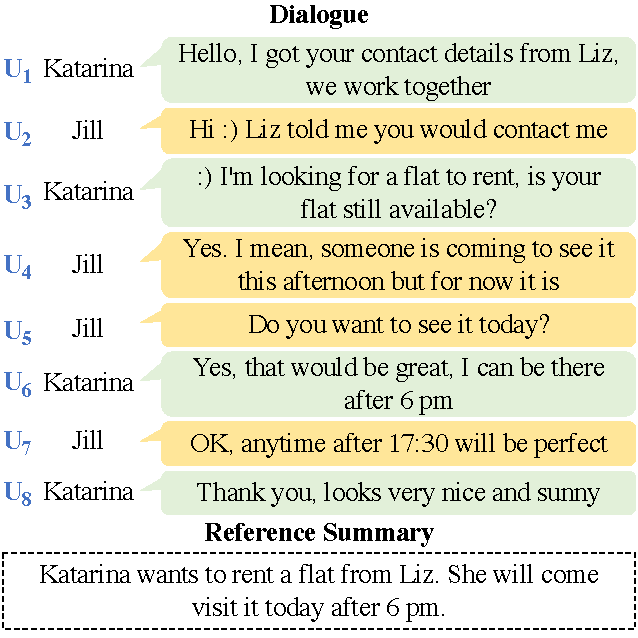
\includegraphics[scale=0.5]{fig/example.pdf}
	\caption{An example multi-party dialogue and its summary. The arrows represent unsequential dependencies between utterances. Elliptical sentences are in italic.}
	\label{fig:example}
\end{figure}

\textbf{Word Level - Language Style and Format:} 
Documents in previous well-researched summarization tasks are written from the third point of view, while dialogues consist of utterances expressed by different speakers in first person. Informal and colloquial expressions are common especially for recorded dialogues from speech, such as ``Whoa'' in $U_6$ and ``u'' representing ``you'' in $U_7$ from Figure~\ref{fig:example}.
Pronouns are frequently used to refer to events or persons mentioned in the dialogue history. Around 72\% of mentions in the conversation are {anaphoras} %pronouns
as stated in \citet{bai2021joint}. Meanwhile, the performance of coreference resolution models trained on normal text drops dramatically on dialogues~\cite{liu2021coreference}. It manifests the existence of language style differences between documents and dialogues, leading to difficulties in understanding the mappings between speakers and events in dialogues.


\textbf{Sentence/Utterance Level - Information Density:}
Document sentences are more self-contained with complete SVO (subject-verb-object) structures, while elliptical utterances are ubiquitous in dialogues, including $U_3$, $U_6$, $U_7$, $U_{11}$ and $U_{12}$.
Besides, the long dialogue can be summarized into a single summary sentence for the example in Figure~\ref{fig:example} as a result of back-and-forth questions and confirmations among speakers for communication purposes.
Question answerings, acknowledgments, and comments~\cite{asher2016discourse} are frequent discourse relations among utterances to narrow down speakers' information gaps and reach agreements.
In this way, dialogue utterances are highly content-dependent, and the information is scattered~\cite{zhang2021exploratory}, raising the difficulties for generating integral contents.

\textbf{Inter-sentence/utterance Level - Discourse structure:}
Articles tend to be well-structured, such as 
general-to-specific structure or deductive order. 
For example, the most important information 
in news summarization are always at the beginning of the document, resulting in a competitive performance of the simple Lead-$3$ baseline~\cite{nallapati2017, see2017get}. However, it is not the same for dialogue summarization. Both Lead-$3$ and Longest-$3$, i.e. $\{U1, U2, U3\}$ and $\{U4, U8, U9\}$ in Figure~\ref{fig:example}, get poor results in different dialogue scenarios~\cite{gliwa2019samsum,chen2021dialsumm,zhang2021emailsum}.
The dependencies among utterances are interleaved, shown by arrows in Figure~\ref{fig:example}, and discourse relations in dialogues are more flexible,
even with the correction of wrong information~\cite{asher2016discourse}. 
For example, 
Jake refused to be available for the reunion in $U_6$, but later agreed
in $U_8$.  As a result, it is more challenging to reason cross utterances for 
dialogue summarization than document summarization.

\textbf{Passage/Session Level - Topic boundaries:} Sentences under the same topic in documents are collected together in a paragraph or a section.
Previous works for extractive~\cite{xiao2019extractive} and abstractive summarization~\cite{cohan2018discourse} both took advantage of such features and made great progress. 
However, a dialogue is a stream of continuous 
utterances without boundaries, even for hours of discussion. The same topic may be discussed repeatedly 
with redundancies and new information, setting up obstacles for content 
selection in dialogue summarization.

%\JQ{it will be good to see the advantages of abstractive vs extractive approaches for dialogue summarization.}
%\JQ{add a little more about extractive methods, and explain why abstractive is more preferred especially in the case of dialogues.}
To better explain why abstractive approaches are more preferred than extractive ones for dialogues, we list the result of the best rule-based extractive baseline, i.e., Longest-$3$~\cite{gliwa2019samsum}, the oracle extractive result determined by Rouge-L Recall score between each summary sentence and dialogue utterances~\cite{chen2018fast}, and the generation by BART fine-tuned on SAMSum dataset~\cite{gliwa2019samsum} of the simple dialogue in Figure~\ref{fig:example} as follows:
\\
\begin{tabular}{|p{1.5cm}|p{\linewidth-2.3cm}|}
	\hline
	\textbf{Longest-$3$} & Jessica: If I move some things around, I can too! Jake: Hell yeah man! You know I freelance, worst case scenario I'll work from wherever we are Jessica: We should meet up where we did last time, it's perfect middle for everyone.\\
	\hline
	\textbf{Oracle} & Jake: Hell yeah man! You know I freelance, worst case scenario I'll work from wherever we are\\
	\hline
	\textbf{BART}& Ted, Pia, Jessica and Jake are going to meet up on Friday night. \\
	\hline
\end{tabular}
\\
We can see that the readability of generated summaries are poor for Longest-$3$ and Oracle due to the language style and format difference. The compression ratio of Longest-$3$ is apparently low while it still misses the involvement of Ted and Pia as a result of low information density of dialogues. Oracle is concise but much more information is missing. Meanwhile, the fine-tuned BART as an abstractive approach shows the favorable performance. Therefore, abstractive approaches becomes the mainstream in researches on dialogue summarization. In a word, dialogue summarization is an valuable research direction in summarization, where the modeling and understanding of dialogues are challenging compared with document summarization and abstractive approaches are especially preferred.
% despite some extractive summarization works~\cite{uma2022comparing,kano2020identifying,bokaei2016extractive}.
%@article{uma2022comparing,
%	title={Comparing Methods for Extractive Summarization of Call Centre Dialogue},
%	author={Uma, Alexandra N and Sityaev, Dmitry},
%	journal={arXiv preprint arXiv:2209.02472},
%	year={2022}
%}

%@inproceedings{kano2020identifying,
%	title={Identifying implicit quotes for unsupervised extractive summarization of conversations},
%	author={Kano, Ryuji and Miura, Yasuhide and Taniguchi, Tomoki and Ohkuma, Tomoko},
%	booktitle={Proceedings of the 1st Conference of the Asia-Pacific Chapter of the Association for Computational Linguistics and the 10th International Joint Conference on Natural Language Processing},
%	pages={291--302},
%	year={2020}
%}

%@article{bokaei2016extractive,
%	title={Extractive summarization of multi-party meetings through discourse segmentation},
%	author={Bokaei, Mohammad Hadi and Sameti, Hossein and Liu, Yang},
%	journal={Natural Language Engineering},
%	volume={22},
%	number={1},
%	pages={41--72},
%	year={2016},
%	publisher={Cambridge University Press}
%}


\subsection{Scenarios for Dialogue Summarization}\label{sec:scenarios}

Considering the source of dialogues and the purpose of doing summarization,
%\KZ{Rephrase this: dialogue sources and summary intentions}, 
we divide the application scenarios into two classes: \textbf{open-domain dialogue summarization (ODS)} and \textbf{task-oriented dialogue summarization (TDS)}. This taxonomy is similar to the one of dialogue systems~\cite{gao2020standard,chen2017survey}.
However, one should note that a pre-defined domain ontology for dialogues is 
not necessarily required for TDS, which is different from that in 
task-oriented dialogue systems.
The application scenarios investigated in previous papers 
are classified into these two classes as shown in Figure~\ref{fig:scenario}.

%\JQ{add citations}
Open-domain dialogue summarization is further divided into daily chat, 
drama conversation, debate \& comment. 
\textbf{Daily chat}~\cite{gliwa2019samsum,chen2021dialsumm} refers to the dialogues happening in our daily lives, 
such as making appointments, discussions between friends, etc. 
\textbf{Drama conversation}~\cite{rameshkumar2020storytelling,zhu2021mediasum,malykh2020sumtitles,chen2021summscreen} represents dialogues from soap operas, 
movies or TV shows, which are dramatized or fabricated with drama scripts 
behind them. Dialogues in these two classes are full of person names 
and events, resulting in narrative summaries about ``who did what''.
\textbf{Debate \& comment}~\cite{misra2015using,fabbri2021convosumm,chowdhury2019cqasumm} focuses more on question answering and 
discussions in online forums and arguments. These dialogues emphasize opinions or solutions to the given subject or questions.

Task-oriented dialogue summarization arises from application scenarios of different domains, which includes but is not limited to customer service, 
law, medical care and official issue.
\textbf{Customer service}~\cite{zou2021topic,feigenblat-etal-2021-tweetsumm-dialog,zhao2021todsum,liu2019automatic,chen2020jddc} refers to conversations between customers and service providers.
Customers start the conversation with their specific intents and agents are required to meet these requirements with the help of their in-domain databases, such as hotel reservations and express information consultation for online shopping. Dialogue summarization for this task is mainly to help service providers quickly go through solutions to users' questions for agent training and service evaluation. 
\textbf{Law}~\cite{fuzw20,duan2019legal,xi2020global} is dialogues related to legal service and 
criminal investigations. Dialogue summarization in this scenario alleviates the recording and summarizing workload 
for law enforcement or legal professionals. 
\textbf{Medical care}~\cite{joshi2020dr,song2020summarizing,song2020summarizing,zhang2021leveraging,liu2019topic} is dialogues between doctors and patients and medical dialogue summarization has some similarity to the research on electronic health records (EHR). Unlike the previous work focusing on mining useful information from EHR~\cite{yadav2018mining}, summarization is to extract useful information from the doctor-patient dialogue and generate an EHR-like or fluent summary for clinical decision-making or online search. It also aims to reduce the burden of domain experts.
\textbf{Official affair}~\cite{carletta2005ami,janin2003icsi,ulrich2008publicly,zhang2021emailsum} is conversations between colleagues for technical or teachers and students for academic issue discussion. They can be either in the format of meetings or e-mails, with summaries covering problems, solutions, and plans.


\begin{figure}
	\centering
	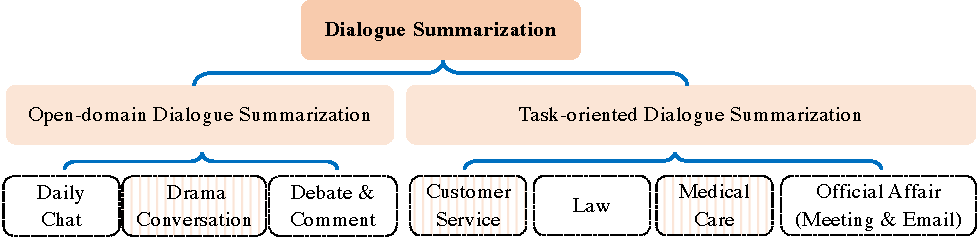
\includegraphics[scale=0.8]{fig/scenarios.pdf}
	\caption{The classification of dialogue summarization tasks with different application scenarios. Datasets proposed for evaluations under each scenario are in Section~\ref{sec:dataset}.}
	\label{fig:scenario}
\end{figure}


We compare and contrast ODS and TDS as follows.
\begin{itemize}
% functional role playing
\item Dialogues happen between \textbf{two or more speakers} both in ODS and TDS, whereas the \textbf{interpersonal relationship} and \textbf{functional relationship} among speakers are different. Generally, speakers in ODS are friends, neighbors, lovers, family members, and so on. 
They are equal either in the aspect of interpersonal relationships or functional relationships. For example, one can raise a question or answer others' questions in online forums~\cite{fabbri2021convosumm}.
In TDS, speakers have different official roles acting for corresponding responsibilities. For example, plaintiff, defendant, witness and judge in court debates~\cite{duan2019legal}, project manager, marketing expert, user interface designer and industrial designer in official meetings~\cite{carletta2005ami} are corresponding roles.
Among different dialogues, roles are the same and can be played by different speakers and a speaker's role is always unchanged for a service platform.
In a word, TDS pays more attention to functional roles while ODS focuses on speakers.


% covering topics
\item Multiple \textbf{topics} may be covered in the same dialogue session.
Topics in ODS are more diverse than in TDS. The summarization models are expected to deal with unlimited open-domain topics such as chitchat, sales, education, and climate at the same time~\cite{chen2021dialsumm}. 
However, topics in TDS are more concentrated and need more expertise for understanding.
Dialogues in TDS either focus on a single domain with more fine-grained topics, such as medical dialogues of different specialties,
or several pre-defined domains, such as restaurant, hotel, and transformation reservation.
Domain knowledge is significant for summarization, and it is divergent across sub-domains. For instance, expertise and medical knowledge are required in doctor-patient dialogues for generating accurate medical concepts~\cite{joshi2020dr} while specific knowledge bases for internal medicine and primary care are not the same.

%  inherent structure
\item The input dialogue for both ODS and TDS is made up of \textbf{a stream of utterance} as defined in Equation~\ref{eq:dialogue}. However, 
the \textbf{structure} of these two types of dialogues are different.
Open-domain dialogues often happen casually and freely while dialogues in TDS may have some inherent working procedures or writing formats. 
For example, the program manager in meetings usually masters the meeting progress~\cite{zhu2020end} implicitly with words such as ``okay, what about ...'', and communications by e-mails consist of semi-structured format including subjects, receivers, senders, and contents~\cite{zhang2021emailsum}. 

% special intentions for summaries
\item \textbf{Focuses of summaries} are distinct. Summaries for ODS in recent research are more like condensed narrative paraphrasing with different levels of granularity. An example is a synopsis from the Fandom wiki\footnote{\url{criticalrole.fandom.com}} maintained by fans for the Critical Role transcripts~\footnote{\url{github.com/RevanthRameshkumar/CRD3}}\cite{rameshkumar2020storytelling}, helping to quickly catch up with what is going on in the long and verbose dialogues. Differently, dialogues in TDS take place with strong intentions for solving problems. Summaries for such dialogues are expected to cover the user intents and corresponding solutions, such as medical summaries for clinical decision making~\cite{joshi2020dr} and customer service summaries for ticket booking~\cite{zhao2021todsum}. As a result, generating faithful content is extremely significant for TDS. %{faithfulness}
\end{itemize}

%\KZ{I feel that just dividing the dialogue summarization into ODS and TDS is a bit
%too coarse-grained. Later when you discuss the approaches, u need to associate
%each approaches with a certain characteristic/scenario of the task. It's more
%useful if u can use some refined characteristics of the task.}

\section{Joint RE Tagging Model}
\label{sec:tagging}

We propose a joint learning model with three modules, namely
sentence representation, RTD and the basic RE tagging, 
as illustrated in \figref{fig:model}. 
Sentence representation module is to encode a sentence to a matrix, which is the 
base of whole model. Other two modules deal with the auxiliary task and 
the main task. Note that superscript ($^S$), ($^R$) and ($^T$) is used
to indicate variables belonging to sentence representation,
RTD and basic RE tagging modules respectively.


\begin{figure}[th]
\centering
\includegraphics[width=\columnwidth]{pictures/model.eps}
\caption{The joint RE tagging model \label{fig:model}}
\end{figure}

\subsection{Sentence Representation Module}
Sentence representation module represents token sequence and extracts low level
features. A sentence $s$ is a sequence of tokens $(w_1, w_2, \ldots, w_i,
\ldots, w_n)$, where $w_i$ is the $i^{th}$ token in $s$, and is represented by
a 1-hot vector $v_i$ with length $|\mathcal{V}|$, where $\mathcal{V}$ is 
the vocabulary. We pretrain word embedding matrix $D$, and use a BiLSTM to
represent a sentence:

\begin{align*}
    \overrightarrow{h}_i^S &= LSTM(\overrightarrow{h}_{i-1}^S, v_iD) \nonumber \\
    \overleftarrow{h}_i^S &= LSTM(\overleftarrow{h}_{i+1}^S, v_iD) \nonumber \\
    h_i^S &= [\overrightarrow{h}_i^S, \overleftarrow{h}_i^S] \nonumber
\end{align*}

Where $\overrightarrow{h}_i^S$ and $\overleftarrow{h}_i^S$ are the hidden state
of forward and backward LSTM. Their concatenation $h_i^S$ is used as the feature
of token $w_i$.


%\subsection{NER Module}
%Typically, NER can also be treated as Tagging problem under ``BIES'' tagging
%scheme \YY{Add some references}. For example, tag sequence ``Person-B Person-E''
%of ``Tim Cook'' indicate that this is a person entity which begins with ``Tim''
%and ends with ``Cook''.
%
%
%
%We decode entity tag sequence using another LSTM. For token
%$w_i$, the input of decoder LSTM, $h_i^S$, is from the sentence module, and the
%output is $h_i^E$. Formally,
%
%\begin{align*}
%  h_i^E &= LSTM(h_{i-1}^E, h_i^S) \nonumber \\
%  p_i^E &= softmax(W^Eh_i^E + b^E) \nonumber
%\end{align*}
%
%$p_i^E$ is the probability vector over NER tag set. Given entity tag sequence,
%all entities can be recovered easily without ambiguity. \YY{Add references}
%
%

\subsection{RTD Module}
The RTD sub-task is similar to RC but detects all relation types in a sentence
without entity information. Different from tagging problem which predicts each
tag on the feature representation of each token, relation type is bounded with
the semantic of whole sentence. We use a CNN to make this multi-label
prediction.

The input of CNN is a feature matrix $H^S$ from sentence module, each column is
the feature vector of corresponding token. Therefore, $H^S$ has two dimension, feature
dimension and sentence length dimension. Considering the linear structural of
sequence, here we choose 1d convolution by treating the feature dimension as
input channels. We
use $K$ kernels to extract sentence level features. The output of $j$th kernel
is $conv_j$. Then max pooling is applied  get the maximum feature value
$pool_j$. The representation of whole sentence $h^R$ is the combination of
$pool_j$ of each kernel. The size of feature vector $h^R$ is the number of
kerners $K$. Here, we can treat each kernel as a feature extractor which is
responsible for some kind of sentence level feature.

\begin{align*}
  H^s &= [h_1^S; h_2^S; \ldots; h_n^S] \nonumber \\
  conv_j &= Relu(kernel_j(H^S)) \nonumber \\
  pool_j^R &= \max(conv_j) \nonumber \\
  h^R &= [pool_1^R, pool_2^R, \ldots, pool_K^R] \nonumber \\
  p_i^R &= sigmoid(W^RH^R + b^R) \nonumber
\end{align*}

To predict relation types, We use a linear layer to convert $h^R$ to label space
vector. Because RTD is a multi-label classification problem, sigmoid function is
chosen as activation function. 
The $k$th element of sigmoid output $p_i^R$ is the
probability of $k$th relation type mentioned in the sentence or not.

\KZ{Add a sentence or two to highlight high level feature fed to
the basic tagging module.}

\subsection{Basic RE Tagging Module}

We use a LSTM to decode the RE tags. The input for 
token $w_i$ is  $h_i^S$ from sentence module, and the output is $h_i^T$. 
$h_i^T$ is a feature representation of token $w_i$, which extracts features by
focusing on the tokens near $w_i$. 
We argue that relation extraction should be based on 
both local and global features. Local features means the
information near by one token while global features means the information of
whole sentence. Obviously, for token $w_i$, the local features can be
represented by $h_i^T$. We use the output $h^R$ of max pooling in the RTD module
as global features, which is a feature representation of the sentence from 
the angle of relation semantic information. 
We call the concatenation of the local features
$h_i^T$ and global features $h^R$,  $h_i^{TR}$, which is used to
predict the tag of $w_i$. Intuitively, mixed features add capabilities to
the decoder. Before predicting the tag by the local features, the decoder can
have a glance at the relation information of the whole sentence. Formally,

\begin{align*}
  h_i^T, c_i^T &= LSTM(h_{i-1}^T, c_{i-1}^T, h_i^S) \nonumber \\
  h_i^{TR} &= [h_i^T, h^R] \nonumber \\
  p_i^T &= softmax(W^Th_i^{TR} + b^T) \nonumber
\end{align*}


\section{Analysis}


For a better understanding of ICL-SC, 
we did comprehensive ablation studies and combined it with the traditional CL. The experiments in this section are done on dialogue summarization, which is representative due to the medium output length.




\subsection{Ablations on the Training Strategy}

%1. strategy: increase; decrease; random
To examine the design of decreasing the prefix for ICL-SC, we introduce the ablation of training strategies as follows:
\begin{itemize}
	\item \textbf{Decrease} refers to the Algorithm~\ref{alg:picl}. Taking $p_{start}=0.6$ and $s=0.3$ as an example, the prefix percentage $p$ varies as $0.6\rightarrow 0.3\rightarrow 0.0$ during training.
	\item \textbf{Increase} means that we gradually increase the length of prefix by increase $p$ following $0.0\rightarrow0.3\rightarrow0.6$.
	\item \textbf{Random} is that we randomly pick $p$ from the set $\{0.0, 0.3, 0.6\}$ in this example.
\end{itemize}

The results are shown in Table~\ref{tab:ablstrategy}, with Decrease ranking first and Increase ranking the worst.
Decrease significantly outperforms other ablations, showing that our sequence completion criterion of shrinking the prefix does work by means of learning from easy to hard.
%, instead of the implicit ``data augmentation'' which calculates different losses given the same sample during training.

\begin{table}[th]
	\scriptsize
	\centering
	\begin{tabular}{cccccc}
		\hline
		{Stra.} & {R1} & {R2} & {RL} & {Met} & {BertS} \\
		\hline
		Decrease &\textbf{53.07} & \textbf{28.23} & \textbf{43.83} & \textbf{26.12} & \textbf{72.17}\\
		Increase & 51.43 & 27.35 & 42.97 & 24.32 & 71.25 \\
		Random & 51.80 & 27.69 & 43.27 & 24.59 & 71.51 \\
		\hline
	\end{tabular}
	\caption{Ablations on ICL strategies. The starting point and the stride are 0.6 and 0.3 respectively.}
	\label{tab:ablstrategy}
\end{table}


\subsection{Parameter Search of the Starting Point and the Stride}

To better understand how the ICL-SC manipulates the difficulty of samples during the training process, we further did experiments on different settings of two newly-introduced hyper-parameters $p_{start}$ and $s$. The results are shown in ~\figref{fig:stridestart}.

\begin{figure}[th]
	\centering
	\begin{minipage}[t]{0.5\linewidth}
		\centering
		\subfloat[Starting Point]{
			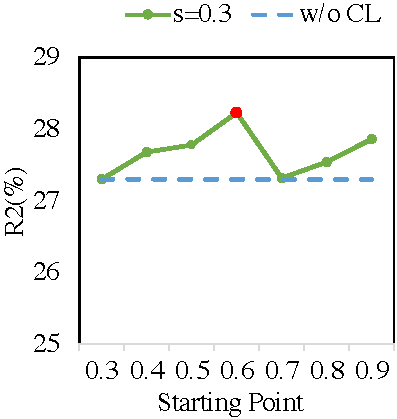
\includegraphics[scale=0.45]{start.pdf}
			%\caption{fig1}
		}%
	\end{minipage}%
	\begin{minipage}[t]{0.5\linewidth}
		\centering
		\subfloat[Stride]{
			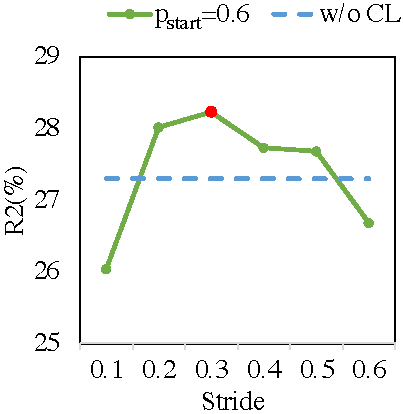
\includegraphics[scale=0.45]{stride.pdf}
			%\caption{fig2}
		}%
	\end{minipage}%
	\centering
	\caption{Parameter search of the starting point $p_{start}$ and the stride $s$. The ``w/o'' CL representing the BART baseline is drawn for comparison.} %Ablations on the starting point of ICL-SC with $s=0.3$ and ablations on the stride of ICL-SC with $p_{start}=0.6$. 
	\label{fig:stridestart}
\end{figure}


We can see that the performance drops with either a too large or too small $p_{start}$. The former one starts training with only predicting the last 1 or 2 tokens according to the average length of reference output shown in Table~\ref{tab:taskdata}. Most of the time, they are punctuation marks that do not carry any important semantic information, leading to a bad warm-up. The latter one requires the model to predict more than half of the output, which are too difficult as a beginning learning target. Besides, a larger $p_{start}$ which is divisible by $s$ achieves more competitive results.
%All of the results still outperforms the original baseline.

The trend is the same for using different stride values. The performance drops with $s$ equaling 0.1 or 0.6. 
The smaller ones lead to too tiny changes, which not only excessively prolongs the required training time but also leads to server outfitting on the training set. The larger ones greatly enlarge the gap between training targets which degrades to 0.0 directly. It also harms the performances.

In a word, the training should start with a medium difficulty training objective and the gap between training objectives shouldn't be too large. Both parameters are closely related to the output length of different tasks. We suggest using ($p_{start}=0.6$, $s=0.3$) for NLG tasks with multi-sentence outputs, and ($p_{start}=0.5$, $s=0.5$) for NLG tasks with single-sentence outputs. All of our experiments are done based on this guideline. %More insights on the relation between the average output length and parameter settings are expected as future work.

%2. hyper-parameters of starting point: 0.6,0.7,0.8,0.9,  0.3,0.4,0.5

%\begin{table}[t]
%	\scriptsize
%	\centering
%	\begin{tabular}{ccccccc}
%		\hline
%		{Start} & {Stride}& {R1} & {R2} & {RL} & {Met} & {BertS} \\
%		\hline
%		0.9 &\multirow{7}{*}{0.3}& 52.97 & 27.86 & {43.72} & \textbf{26.23} & 71.89 \\
%		0.8 & &52.54 & 27.54 & 43.44 & 26.08 & 71.92 \\
%		0.7 & &52.46 & 27.32 & 43.32 & 25.26 & 71.32\\
%		0.6 & &\textbf{53.07} & \textbf{28.23} & \textbf{43.83} & 26.12 & \textbf{72.17}\\
%		0.5 & &52.37 & 27.78 & 43.54 & 25.31 & 71.74 \\
%		0.4 & &52.14 & 27.68 & 43.20 & 25.09 & 71.52 \\
%		0.3 & &51.46 & 27.30 & 42.74 & 24.37 & 71.15\\
%		\hline
%		\multirow{6}{*}{0.6}&0.1  & 50.75 & 26.04 & 41.86 & 24.06 & 70.81\\
%		&0.2 & 52.46 & 28.02 & 43.63 & 25.21 & 71.79\\
%		&0.3 & \textbf{53.07} & \textbf{28.23} & \textbf{43.83} & \textbf{26.12} & \textbf{72.17} \\
%		&0.4 & 51.90 & 27.73 & 43.09 & 25.11 & 71.53\\
%		&0.5 & 51.84 & 27.68 & 43.15 & 24.99 &71.73\\
%		&0.6 & 50.86 & 26.68 & 42.32 & 23.55 &70.76\\
%		\hline
%		w/o & w/o &51.88 & 27.30 & 42.77 & 24.75 & 71.38 \\
%		\hline
%	\end{tabular}
%	\caption{Ablations on the starting point of propotional ICL with the stride equaling 0.3 and ablations on the stride of propotional ICL with the starting point equaling 0.6. The last line with ``w/o'' representing the BART baseline without using the ICL strategy is listed for comparison.}
%	\label{tab:ablstart}
%\end{table}


\subsection{Combinations with the Traditional CL}


We design $4$ different traditional CL strategies % and rank samples in the training set 
for dialogue summarization empirically as follows:
\begin{itemize}
	\item \textbf{Input length (InLen)} refers to the number of tokens in the input dialogue. The longer a dialogue is, the more complex a sample is.
	\item \textbf{Output length (OutLen)} is the number of tokens in a reference summary, which is also proportional to the difficulty of a sample.
	\item \textbf{Compression ratio (CompR)} equals the output length divided by the input length. More compressed training pairs are harder.% for models to learn from. %We generally agree that 
	\item \textbf{Abstractiveness (Abstr)} represents the percentage of novel words in the reference summary which are not in the dialogue. We measure it by Rouge-2 recall, which is inversely proportional to the difficulty level.
\end{itemize}

\begin{table}[t]
	\scriptsize
	\centering
	\begin{tabular}{lccccc}
		\hline
		{Method} & {R1} & {R2} & {RL} & {Met} & {BertS} \\
		\hline
		w/o CL & 51.88 & 27.30 & 42.77 & 24.75 & 71.38 \\
		\hline
		InLen & 52.19 & \textbf{27.73} & \textbf{43.50} & 25.57 & 71.73\\
		InLen+ & \textbf{52.56} & 27.60 & 43.43 & \textbf{25.77} & \textbf{71.92}\\
		\hline
		OutLen & 41.38 & 20.88 & 31.77 & \textbf{27.95} & 67.21\\
		OutLen+ &\textbf{43.96} & \textbf{22.14} & \textbf{33.05} & 26.39 & \textbf{67.64} \\
		\hline
		CompR & 39.68 & 19.28 & 34.73 & 14.41 & 65.96 \\
		CompR+ & \textbf{41.59} & \textbf{20.78} & \textbf{36.62} & \textbf{15.22} & \textbf{67.19}\\
		\hline
		Abstr & \textbf{44.61} & 20.10 & 36.93 & \textbf{17.34} & 68.29 \\
		Abstr+ & 44.41 & \textbf{20.64} & \textbf{37.29} & 17.25 & \textbf{68.33} \\
		\hline
	\end{tabular}
	\caption{Performaces with traditional CL strategies. ``+'' represents experiments further armed with ICL-SC.}
	\label{tab:traditional}
\end{table}
The results based on the ordered training samples according to these intuitive CL strategies are shown in Table~\ref{tab:traditional}. It shows that only InLen improves the vanilla model, but it still lags behind our results in Table~\ref{tab:end2endds}. Other strategies failed mainly due to the low data quality at the beginning or the end of training. 
Taking Abstr as an example, samples with the highest 
Rouge-2 recall are gathered at the beginning where 
their inputs and outputs are almost the same. 
This leads to a bad initialization for models learning 
the summarization ability. 

Besides, some strategies 
are incompatible, such as OutLen and CompR. Samples with the shortest output length are always too compressed. Therefore, it's hard to develop a comprehensive score for a better ranking. It should be also noticed that most of these strategies are developed for dialogue summarization, which are not suitable for generalization. In a word, it's hard to develop a 
comprehensive strategy for one task or a unified strategy for different NLG tasks with traditional CL. 

%Our ICL-SC can be easily combined with these CL strategies. %by training with ordered training samples instead of random sampling. 
ICL-SC not only outperforms these CL strategies, but also improves them when easily combined. 

\label{sec:tracl}


%\subsection{Performance on Variable Lengths}

%\begin{table}
%	\small
%	\centering
%	\begin{tabular}{lcccccc}
%	\hline
%	Dataset &  Avg & Std & \#1 & \#2 & \#3 & \#4 \\
%	\hline
%	DREAM & 5.59 & 2.61 & 483 & 653 & 468 & 483 \\
%	\hline
%	SAMSum & 24.99 & 13.06 & 227 & 260 & 170 & 162 \\	
%	\hline
%	\multirow{2}{*}{Shakespeare} & 12.24 & 9.27 & 423 & 288 & 290 & 461 \\
%	& 11.02 & 7.10 & 423 & 328 & 264 & 447 \\
%	\hline
%	SQuAD1.1 & 13.09 & 4.27 & 2330 & 4755 & 3041 & 1751 \\
%	\hline
%	CNNDM & \\
%	\hline
%	\end{tabular}
%	\caption{Statistics on variable output length. Avg and Std refer to the average and the standard deviation of the output length. \#1 to \#4 represent the number of samples belonging to different test buckets divided by the output length in ascending order.
%	Shakespeare contains two rows as its output can be in both styles.}
%	\label{tab:ablength}
%\end{table}

%\begin{figure*}[th]
%	\centering

%		\begin{minipage}[t]{0.5\linewidth}
%			\centering
%				\subfloat[Dialogue Summarization]{
%			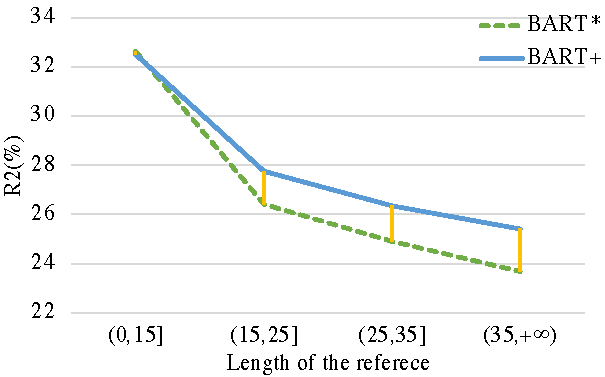
\includegraphics[scale=0.65]{length-ds.pdf}
%\caption{fig1}
%				}%
%		\end{minipage}%
%		\begin{minipage}[t]{0.5\linewidth}
%			\centering
%				\subfloat[Reading Comprehension]{
%			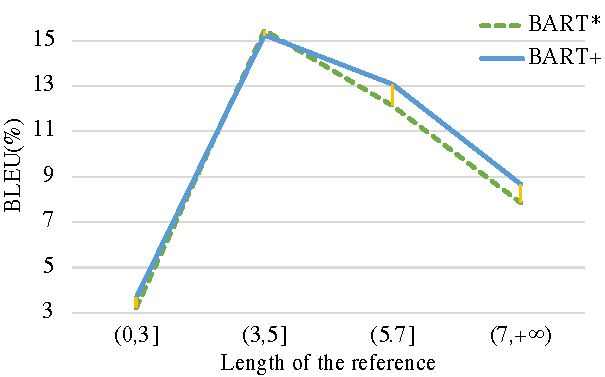
\includegraphics[scale=0.65]{length-rc.pdf}
%\caption{fig2}
%				}%
%		\end{minipage}%

%		\begin{minipage}[t]{0.5\linewidth}
%			\centering
%			\subfloat[Style Transfer]{
%				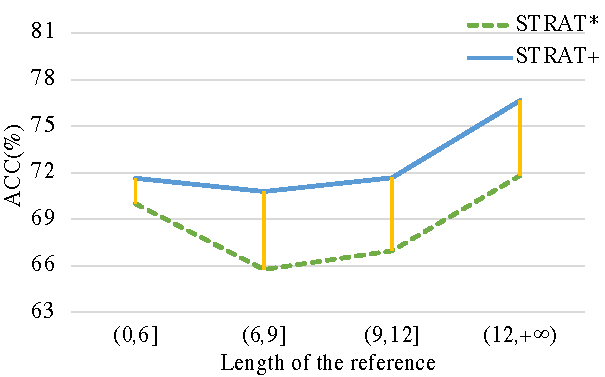
\includegraphics[scale=0.65]{length-st.pdf}
%\caption{fig2}
%			}%
%		\end{minipage}%
%		\begin{minipage}[t]{0.5\linewidth}
%			\centering
%			\subfloat[Question Generation]{
%				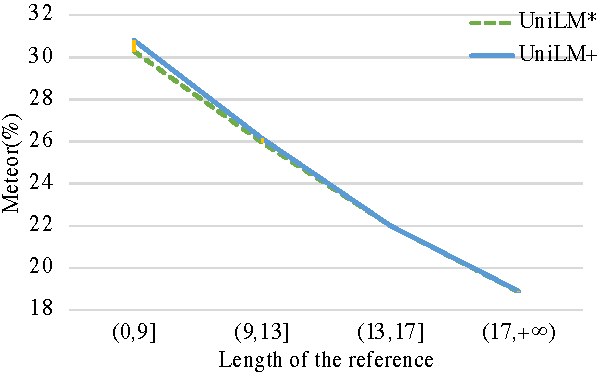
\includegraphics[scale=0.65]{length-qg.pdf}
%\caption{fig2}
%			}%
%		\end{minipage}
%	\centering
%	\caption{Comparisons on variable lengths. \KZ{The label should read
%Length of the ``reference'' text.}}
%	\label{fig:ablength}
%\end{figure*}






\section{Conclusion}

In this paper, we incorporated the idea of Cookie Theft picture description task into the evaluation of the high-level cognitive abilities of LVLMs and designed a novel evaluation benchmark called CogBench.
% Images in CogBench are of high quality and require more cognitive reasonings to understand, which makes it different from existing image datasets.
The images in CogBench are of high quality and demand more complex cognitive reasoning for interpretation, setting it apart from existing image datasets.
% It consists of a image description task and a VQA task.
Experiments show that there is still a large gap between the cognitive abilities of LVLMs and human beings, indicating CogBench is a challenging benchmark.

% In the future


\bibliography{emnlp-ijcnlp-2019}
\bibliographystyle{acl_natbib}

\end{document}
